\section{Simulación} \label{sec:simulacion}

Siguiendo el tutorial comenzamos ensamblando nuestro robot, y marcando sus ejes dentro del programa de SolidWorks.

\begin{figure}[h]
	\centering
	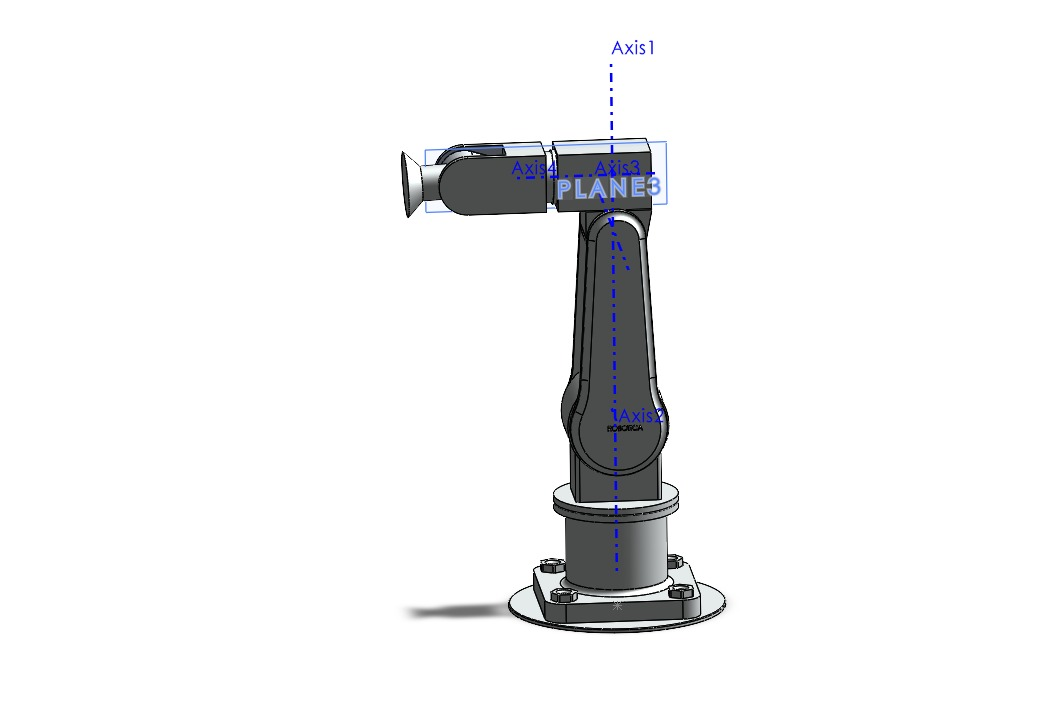
\includegraphics[width=\linewidth]{img/ROBOT SOLID}
	\caption{Robot ensamblado en SolidWorks}
	\label{fig:ROBOT SOLID}
\end{figure}














Aquí pueden de forma resumida los pasos que vienen en el tutorial. Pueden hacer referencia a \href{https://github.com/IvanMedinaGL/Robotica}{mi repositorio} \cite{medinagl_robotica}. Sería la parte de dónde obtuvieron el modelo del robot, cómo lo exportaron de \textit{SolidWorks} a \textit{URDF}, cómo usaron \textit{Ubuntu}, ya sea con una máquina virtual (como \textit{VirtualBox}) o con \textit{Windows Subsystem for Linux} (WSL), cómo simularon que las dos pinzas se muevan al mismo tiempo, si le metieron electroimán o lo intentaron y cómo, el cómo cambiaron los controladores, cómo lo ejecutaron y las herramientas necesarias (como RViz, Gazebo, MoveIt...), etc.